
%% Warning: section is very new, and likely subject to errors
% TODO: Write final section


\subsection{Integrals}
Say we've got a function. This function can be expressed as a line on a graph. This line separates the graph in two sections; one above and one below the line.

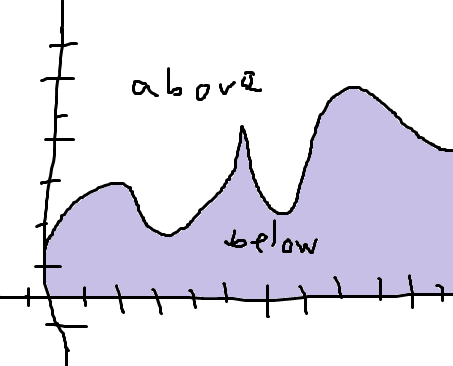
\includegraphics{integralGraph_sketch}
TODO: prettify graph pic

How much space exists below the line?

\subsubsection{Setting up the Language}
A problem like the one described above is normally solved with an integral. To solve an integral, we'll first need a language that can describe the function(which in turn describes the line).

Unlike complex numbers, there is no one uniform expression that can describe any function. Thus, this time, we'll have to invent something a little bit more flexible.

\begin{minted}{haskell}
data Funk = X
  | Constant Double
  | Add Funk Funk
  | Multiply Funk Funk
  deriving (Show)
\end{minted}

We'll do something a little more standard this time. The above DSL mimics the standard syntax for functions, or at least as closely as we can make it. Our ''words'' are the variable X, a constant, addition, and multiplication.

These are theoretically used in the exact same way that they would be on paper; the first two are values, while the second two are operators. For simplicity's sake, we'll be using an integer to describe our constants. X is, as you'd expect, an undefined variable.

Our operators; addition and multiplication, are a little more complicated. Rather than being simple values, they are statements that take other ''words'' and tie them together. Perhaps this is best explained by an example. Say you want the function ''$5 + x^2$''. In our DSL, we'd write it as
\begin{minted}{haskell}
test :: Funk
test = Add (Constant 5) (Multiply X X)
\end{minted}

The Multiply word, in this case, ties two X's together, while the Add word ties the result to the constant. Thus, we've created a ''sentence'' of words(or a function, according to math).

This is still a very limited language. At some point, we'll probably want more words to describe any other operations we might want to be part of our calculations; powers, divisions, roots, etc. The list is effectively endless, and so to keep things comprehensive, let's stick to this simplified version for now.

\paragraph{} We're still not ready for integrals, however. First, we'll also need a function that takes the sentences we just created plus a value for x and produces a result. In practice, this is simplicity itself; we'll simply replace each word with their algebraic equivalent and let Haskell roleplay as a calculator for a moment. To wit:
\begin{minted}{haskell}
-- calculate
--input: function, value for X
--output: result
calculate :: Funk -> Double -> Double
calculate X value                       = value
calculate (Constant num) value          = num
calculate (Add funk1 funk2) value       = (calculate funk1 value) + (calculate funk2 value)
calculate (Multiply funk1 funk2) value  = (calculate funk1 value) * (calculate funk2 value)
\end{minted}

\begin{exercise}
Expand the DSL with a word for subtraction, and full functionality in the 'Calculate' operator. 
\end{exercise}


\subsubsection{Brute Force Mathematics}
Right, with our basic language defined, it's time to take a first stab at that graph.

The traditional first step to solving an integral is to, instead of look for an entirely accurate answer, instead look for an estimated answer.

To wit, let's use our test function from above (5 + $x^2$), and say we want to know how much space exists beneath the line and between x=2 and x=5. To do this, we could take the average of these numbers, (2+5)/2=3.5, and see how much space would exist between the line if this average was true throughout the function.
\begin{minted}{haskell}
-- bfIntegral (brute force integral)
--input: function, startvalue, stopvalue
--output: result
bfIntegral :: Funk -> Double -> Double -> Double
bfIntegral funk start stop = (calculate funk ((start+stop)/2)) * (stop-start)
\end{minted}

There, quick and easy. Sadly not accurate. Our main problem is that our test function does not grows linearly. This means that taking a value ''in the middle'' of the graph and expecting the values on either side to balance each other out is foolish.

Rather than despair, however, let's try to make our integral a little more accurate. The way we go about this is that rather than use an average for the entire graph, we cut the problem into equally sized chunks, calculate each chunk individually, and add the results together.

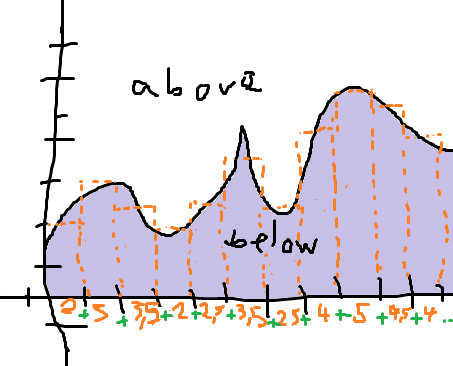
\includegraphics{integralBruteForce_sketch}
TODO: prettify picture of basic integral.

\begin{minted}{haskell}
-- bfIntegral' (brute force integral alternative)
--input: function, start, end
--output: result
bfIntegral' :: Funk -> Double -> Double -> Double
bfIntegral' funk start end
  | start >= end = 0
  | otherwise    = (calculate funk start) + (bfIntegral' funk (start+1) end)
\end{minted}
We made each chunk precisely 1 wide for simplicity, using a simple recursive function. The result should be considerably more accurate now, though still not perfect.

We also learnt an important lesson. See, the first example used chunks as well. Or rather, a single chunk. By cutting the chunk into smaller chunks, we increased accuracy. This is something we can repeat. In theory, we can repeat this infinitely; cutting our problem into an infinite number of infinitely small chunks. If each size reduction on the part of the chunks brings us closer to the true answer, and we reduce the size infinitely, then we will become infinitely close to the true answer. I.E. We will have the true answer.

\paragraph{} In practice, no computer can actually calculate infinity, but they can get close enough for most purposes. So let's give that a shot and see what happens; let's make one chunk for every 1/100.
\begin{minted}{haskell}
-- bfIntegral'' (brute force integral: electric boogaloo)
--input: function, start, stop
--output: result
bfIntegral'' :: Funk -> Double -> Double -> Double
bfIntegral'' funk start end
  | start >= end = 0
  | otherwise    = (calculate funk start)*0.01 + (bfIntegral'' funk (start+0.01) end)
\end{minted}
 If this is still not enough.. well, there's still one subsection left to read. Beware though, it might be math heavy.

\subsubsection{An Elegant yet Primitive Solution}
TODO convert to primitive function solution goes here

\begin{exercise}
Extend support for subtraction to this form of integral.
\end{exercise}
\begin{exercise}
Expand the DSL with a word for a complex constant, plus associated functionality for both types of integral.
\end{exercise}